% To convert to svg
% lualatex --output-format=dvi mother.tex
% dvisvgm mother.dvi
% \documentclass[dvisvgm]{minimal}		%uncomment to convert to svg

\documentclass[border=0]{standalone}
\usepackage{tikz}
\usetikzlibrary{calc,shapes.geometric}
\usepackage{xcolor}
\definecolor{highlight2}{HTML}{99cc99}
\begin{document}
    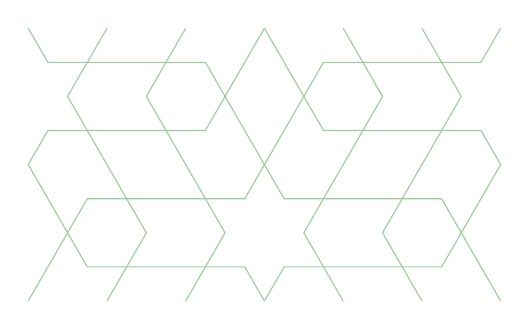
\begin{tikzpicture}
        \pgfmathsetmacro{\a}{sqrt(3)}
        \foreach \x in {0,1}{
            \draw[highlight2] ($(60:1)!.5!(120:1)$)--++({-120+\x*60}:1)--++({-60-\x*60}:1.5)--++(\x*180:2)--++({-60-\x*60}:1.5);
            \draw[highlight2] ($(1*60:1)!.5!(120:1)$)++({-120+\x*60}:1)--++({120-\x*60}:0.5)--++({180-\x*180}:2)--++({120-\x*60}:0.5);
            \draw[highlight2] ($(1*60:1)!.5!(120:1)$)++({-120+\x*60}:1)--++({-120+\x*60}:0.5)--++({180-\x*180}:2)--++({-120+\x*60}:0.5);
            \draw[highlight2] ({120-\x*60}:1)++({180-\x*180}:.5)--++({-120+\x*60}:1)--++({-60-\x*60}:2)--++({-120+\x*60}:0.5)--++(\x*180:0.5)--++({-60-\x*60}:0.5);
            \draw[highlight2] ({120-\x*60}:1)++({180-\x*180}:1.5)--++({-120+\x*60}:1)--++({-60-\x*60}:2)--++({-120+\x*60}:1);
            \draw[highlight2] (-90:\a)++({-150+\x*120}:\a/2)--++({-120+\x*60}:0.5);
            \draw[highlight2] (-90:\a)++({-150+\x*120}:\a/2)--++({180-\x*180}:1.5)--++({120-\x*60}:1.5);
            }
    \end{tikzpicture}
\end{document}
